\section{METODOLOGI}

Penelitian ini dilaksanakan sesuai dengan blok diagram pada Gambar 3.1. Blok
diagram tersebut merupakan metodologi penelitian yang disusun sesuai dengan langkah-
langkah yang dilakukan dalam penelitian.

\begin{figure} [ht] \centering
  \counterwithin{figure}{section}
  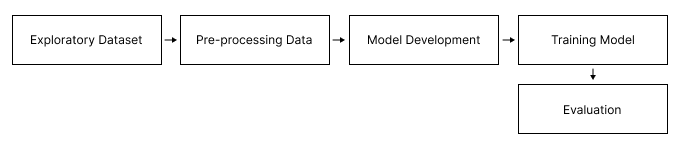
\includegraphics[width=160mm]{gambar/metodologi.png}
  \caption{Metodologi Penelitian}
\end{figure}

\subsection{Desain Roket yang Digunakan}


% Contoh input gambar dengan format *.jpg
\begin{figure} [ht] \centering
  % Nama dari file gambar yang diinputkan
  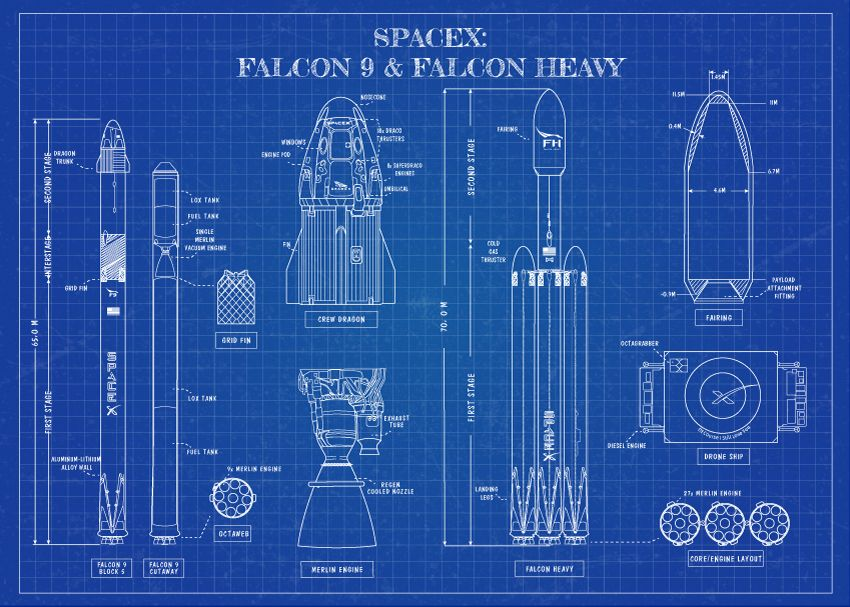
\includegraphics[scale=0.45]{gambar/blueprint.jpg}
  % Keterangan gambar yang diinputkan
  \caption{\emph{Blueprint} roket yang akan diuji coba \citep{SpaceXBlueprint}}
  % Label referensi dari gambar yang diinputkan
  \label{fig:Blueprint}
\end{figure}

% Contoh penggunaan referensi dari gambar yang diinputkan
Pada \emph{blueprint} yang tertera di Gambar \ref{fig:Blueprint}. \lipsum[12]

\subsection{Perhitungan Energi Roket}

\lipsum[13]

\subsection{Mekanisme Pengujian}

\lipsum[14]
